\chapter{Architecture and System Design}

	System architecture can be divided into three sub-systems :
	\begin{itemize}
		\item 	 Web server
		\item 	 Android application
		\item 	 Database
	\end{itemize}
		
		\textbf{Android application}
		 It allows user to view and interact with the specific components of the graphic interface. In Android, graphical components are written in the XML (Extensible Markup Language) which is the language that can be understood by human and by the machine. On interaction with the GUI elements certain parts of the Android code are executed, mostly the ones that send HTTP requests to the Web Server. To send HTTP requests we are using Android’s Volley library.

		\textbf{Web Server}
		 Web Server is the one who responds to the HTTP requests that are sent by Android application. Primary task of the web server is communication with the client (Android application) and fetching data from the database. Required data is then sent back to the client that displays data on the GUI. Response can be sent in the JSON (JavaScript Object Notation) format or as the plain String. Web server is also the one responsible for authentication and authorization of the user, server checks if the user has permission to access the certain data. If user does not have the required permission, Server will send Error response back to the client whose task is to handle the error properly.

		 Programming language in which we have coded the Android application is Java, GUI components are written in the XML language and server-side code is written in Python. IDE (Integrated development environment) we are using is Android Studio for the client-side code and IDLE for the server-side code.

		 Design pattern we are using is MVC(Model-View-Controller). It is a common architectural pattern which is used to design and create interfaces and the structure of an application. This pattern divides the application into three parts that are dependent and connected to each other. These designs are used to distinguish the presentation of data from the way the data is accepted from the user to the data that is being shown. 
		 MVC design pattern consists of: 
			
		\begin{itemize}
			\item 	 Model
			\item 	 View
			\item 	 Controller		
		\end{itemize}

		\textbf{Model}
		 The Model component corresponds to all the data-related logic that the user works with. This can represent either the data that is being transferred between the View and Controller components or any other business logic-related data. For example, a Customer object will retrieve the customer information from the database, manipulate it and update it data back to the database or use it to render data. 
		In Android application Model is usually represented as independent Java class that contains data about e.g. Customer. That data is the one that is kept in the data base and displayed in the View component. 

		\textbf{View}
		 The View component is used for all the UI logic of the application. For example, the Customer view will include all the UI components such as text boxes, dropdowns, etc. that the final user interacts with. 
		In our application an example of View would be Activity for register, user interacts with the View, enters the necessary information that are then transferred to the Model and finally to the database via Controller.

		\textbf{Controller}
		 Controllers act as an interface between Model and View components to process all the business logic and incoming requests, manipulate data using the Model component and interact with the Views to render the final output. For example, the Customer controller will handle all the interactions and inputs from the Customer View and update the database using the Customer Model. The same controller will be used to view the Customer data.
\pagebreak
				
		\section{Database}
			
			
		 Database used for this project is a relation based database made in SQLite. Relation is usually referred to as a table that has tuples. Tuple is an object that represents an information. Purpose of the database is easy and fast data manipulation, including saving, deleting, updating and sending data to the server. Database has relations:
		\begin{itemize}
			\item 	 User
			\item 	 Festival
			\item 	 Event
			\item 	 Specialization
			\item 	 WorkerSpec
			\item 	 Auction
			\item 	 Application
			\item 	 Job
			\item 	 JobSpec
			\item 	 FestivalOrganizers
		\end{itemize}
		\pagebreak
			\subsection{Tables details}
			

				\textbf{User}  has entities for every user of the app. It has all needed personal information about the user and his role.
				
				\begin{longtabu} to \textwidth {|X[6, l]|X[6, l]|X[20, l]|}
					
					\hline \multicolumn{3}{|c|}{\textbf{User}}	 \\[3pt] \hline
					\endfirsthead
					
					\hline 
					\endlastfoot
					
					\cellcolor{LightGreen}user\_id & INT	&  	User identification number 	\\ \hline
					username	& VARCHAR &  Unique username 	\\ \hline 
					password & VARCHAR & User account password  \\ \hline 
					firstname & VARCHAR	&  Users first name	\\ \hline 
					lastname & VARCHAR	&  Users last name	\\ \hline 
					picture & VARCHAR	&  Profile picture string	\\ \hline 
					phone & VARCHAR	&  Users phone number	\\ \hline 
					email & VARCHAR	&  Users email address	\\ \hline 
					role & VARCHAR	&  Role user will persue in application	\\ \hline
					
				\end{longtabu}

				\textbf{Festival}  contains all needed information about the festival.
				
				\begin{longtabu} to \textwidth {|X[6, l]|X[6, l]|X[20, l]|}
					
					\hline \multicolumn{3}{|c|}{\textbf{Festival}}	 \\[3pt] \hline
					\endfirsthead

					\hline 
					\endlastfoot
					
					\cellcolor{LightGreen}festival\_id & INT	&  	Festival identification number 	\\ \hline
					\cellcolor{LightBlue}creator\_id	& INT &  ID of the user who created the festival 	\\ \hline 
					name & VARCHAR & Festival name  \\ \hline 
					desc & VARCHAR	&  Short festival description, can be empty	\\ \hline 
					logo & VARCHAR	&  Festivals logo string	\\ \hline 
					duration & INTERVAL	&  Festival duration interval	\\ \hline 
					active & BOOLEAN	&  True if festival is active, False if it's unactive	\\ \hline 
					
				\end{longtabu}

				\textbf{Event}  contains information about the event of the festival.
				
				\begin{longtabu} to \textwidth {|X[6, l]|X[6, l]|X[20, l]|}
					
					\hline \multicolumn{3}{|c|}{\textbf{Event}}	 \\[3pt] \hline
					\endfirsthead
					
					\hline 
					\endlastfoot
					
					\cellcolor{LightGreen}event\_id & INT	&  	Event identification number 	\\ \hline
					\cellcolor{LightBlue}festival\_id	& INT &  ID of the festival that event belongs to 	\\ \hline 
					\cellcolor{LightBlue}organizer\_id 	& INT &  ID of the user who created the event  	\\ \hline 
					name & VARCHAR & Event name  \\ \hline 
					desc & VARCHAR	&  Short event description, can be empty	\\ \hline 
					location & VARCHAR	&  Events location	\\ \hline 
					start\_Time & TIMESTAMP	&  Event start time	\\ \hline 
					end\_Time & TIMESTAMP	&  Event end time  \\ \hline 
					
				\end{longtabu}


				\textbf{Specialization}  contains all different specializations and their names.
				
				\begin{longtabu} to \textwidth {|X[7, l]|X[6, l]|X[19, l]|}
					
					\hline \multicolumn{3}{|c|}{\textbf{Specialization}}	 \\[3pt] \hline
					\endfirsthead
					
					\hline 
					\endlastfoot
					
					\cellcolor{LightBlue}specialization\_id & INT	&  	Specializations identification number 	\\ \hline
					name & VARCHAR & Name of the specialization \\ \hline

					
				\end{longtabu}

				\textbf{WorkerSpec}  contains specifications about the user who wants to apply as a worker and his specializations.
				
				\begin{longtabu} to \textwidth {|X[7, l]|X[6, l]|X[19, l]|}
					
					\hline \multicolumn{3}{|c|}{\textbf{WorkerSpec}}	 \\[3pt] \hline
					\endfirsthead
					
					\hline 
					\endlastfoot
					
					\cellcolor{LightGreen}worker\_id & INT	&  	Workers identification number 	\\ \hline
					\cellcolor{LightBlue}specialization\_id & INT	&  	Specializations identification number 	\\ \hline

					
				\end{longtabu}

				\textbf{Auction}  contains information about auctions.
				
				\begin{longtabu} to \textwidth {|X[6, l]|X[6, l]|X[20, l]|}
					
					\hline \multicolumn{3}{|c|}{\textbf{Auction}}	 \\[3pt] \hline
					\endfirsthead
					
					\hline 
					\endlastfoot
					
					\cellcolor{LightGreen}auction\_id & INT	&  	Auction identification number 	\\ \hline
					start\_Time & TIMESTAMP	&  Auction start time	\\ \hline 
					end\_Time & TIMESTAMP	&  Auction end time  \\ \hline 
					
				\end{longtabu}


				\textbf{Application}  contains information about applications for auctions.
				
				\begin{longtabu} to \textwidth {|X[8, l]|X[6, l]|X[18, l]|}
					
					\hline \multicolumn{3}{|c|}{\textbf{Application}}	 \\[3pt] \hline
					\endfirsthead
					
					\hline \multicolumn{3}{|c|}{\textbf{Application}}	 \\[3pt] \hline
					\endhead
					
					\hline 
					\endlastfoot
					
					\cellcolor{LightGreen}application\_id & INT	&  	Application identification number 	\\ \hline
					\cellcolor{LightBlue}auction\_id & INT	&  	Auction identification number that worker applies for 	\\ \hline
					\cellcolor{LightBlue}worker\_id & INT	&  	Workers identification number 	\\ \hline
					price & FLOAT & Offered pay for the job \\ \hline
					comment & VARCHAR & Additional comment for application, can be empty \\ \hline
					approximate\_time & INT & Time needed to complete the job, in days \\ \hline
					number\_of\_people & INT & Number of people that will be doing the job \\ \hline

					
				\end{longtabu}
			

				\textbf{Job}  contains information about jobs that had an auction.
				
				\begin{longtabu} to \textwidth {|X[6, l]|X[6, l]|X[20, l]|}
					
					\hline \multicolumn{3}{|c|}{\textbf{Job}}	 \\[3pt] \hline
					\endfirsthead
					
					\hline \multicolumn{3}{|c|}{\textbf{Job}}	 \\[3pt] \hline
					\endhead
					
					\hline 
					\endlastfoot
					
					\cellcolor{LightGreen}job\_id & INT	&  	Job identification number 	\\ \hline
					\cellcolor{LightBlue}event\_id & INT	&  	Events identification number that job is for\\ \hline
					\cellcolor{LightBlue}worker\_id & INT	&  	Workers identification number that does the job\\ \hline
					\cellcolor{LightBlue}auction\_id & INT	&  	Auctions identification number that auctioned the job\\ \hline
					start\_Time & DATETIME	&  Jobs start time	\\ \hline 
					is\_Completed & BOOLEAN	&  True if job is finished, false if it's still active \\ \hline 

				
				\end{longtabu}


				\textbf{JobSpec}  contains specializations that are needed for the job.
				
				\begin{longtabu} to \textwidth {|X[7, l]|X[6, l]|X[19, l]|}
					
					\hline \multicolumn{3}{|c|}{\textbf{JobSpec}}	 \\[3pt] \hline
					\endfirsthead
					
					\hline \multicolumn{3}{|c|}{\textbf{JobSpec}}	 \\[3pt] \hline
					\endhead
					
					\hline 
					\endlastfoot
					
					\cellcolor{LightGreen}job\_id & INT	&  	Job identification number 	\\ \hline
					\cellcolor{LightBlue}specialization\_id & INT	&  	Specializations identification number 	\\ \hline

					
				\end{longtabu}


				\textbf{FestivalOrganizers}  contains information which user, that is also an organizer, applied for which festival.
				
				\begin{longtabu} to \textwidth {|X[6, l]|X[6, l]|X[20, l]|}
					
					\hline \multicolumn{3}{|c|}{\textbf{FestivalOrganizers}}	 \\[3pt] \hline
					\endfirsthead
					
					\hline 
					\endlastfoot
					
					\cellcolor{LightGreen}festival\_id & INT	&  	Festival identification number 	\\ \hline
					\cellcolor{LightGreen}organizer\_id & INT	&  	Organizers identification number 	\\ \hline
					status & INT	&  \-1 when organizer is waiting on leader, 0 when rejected and 1 when accepted \\ \hline 

				
				\end{longtabu}
			\pagebreak
			\subsection{Database diagrams}
				
				
				\begin{figure}[H]
					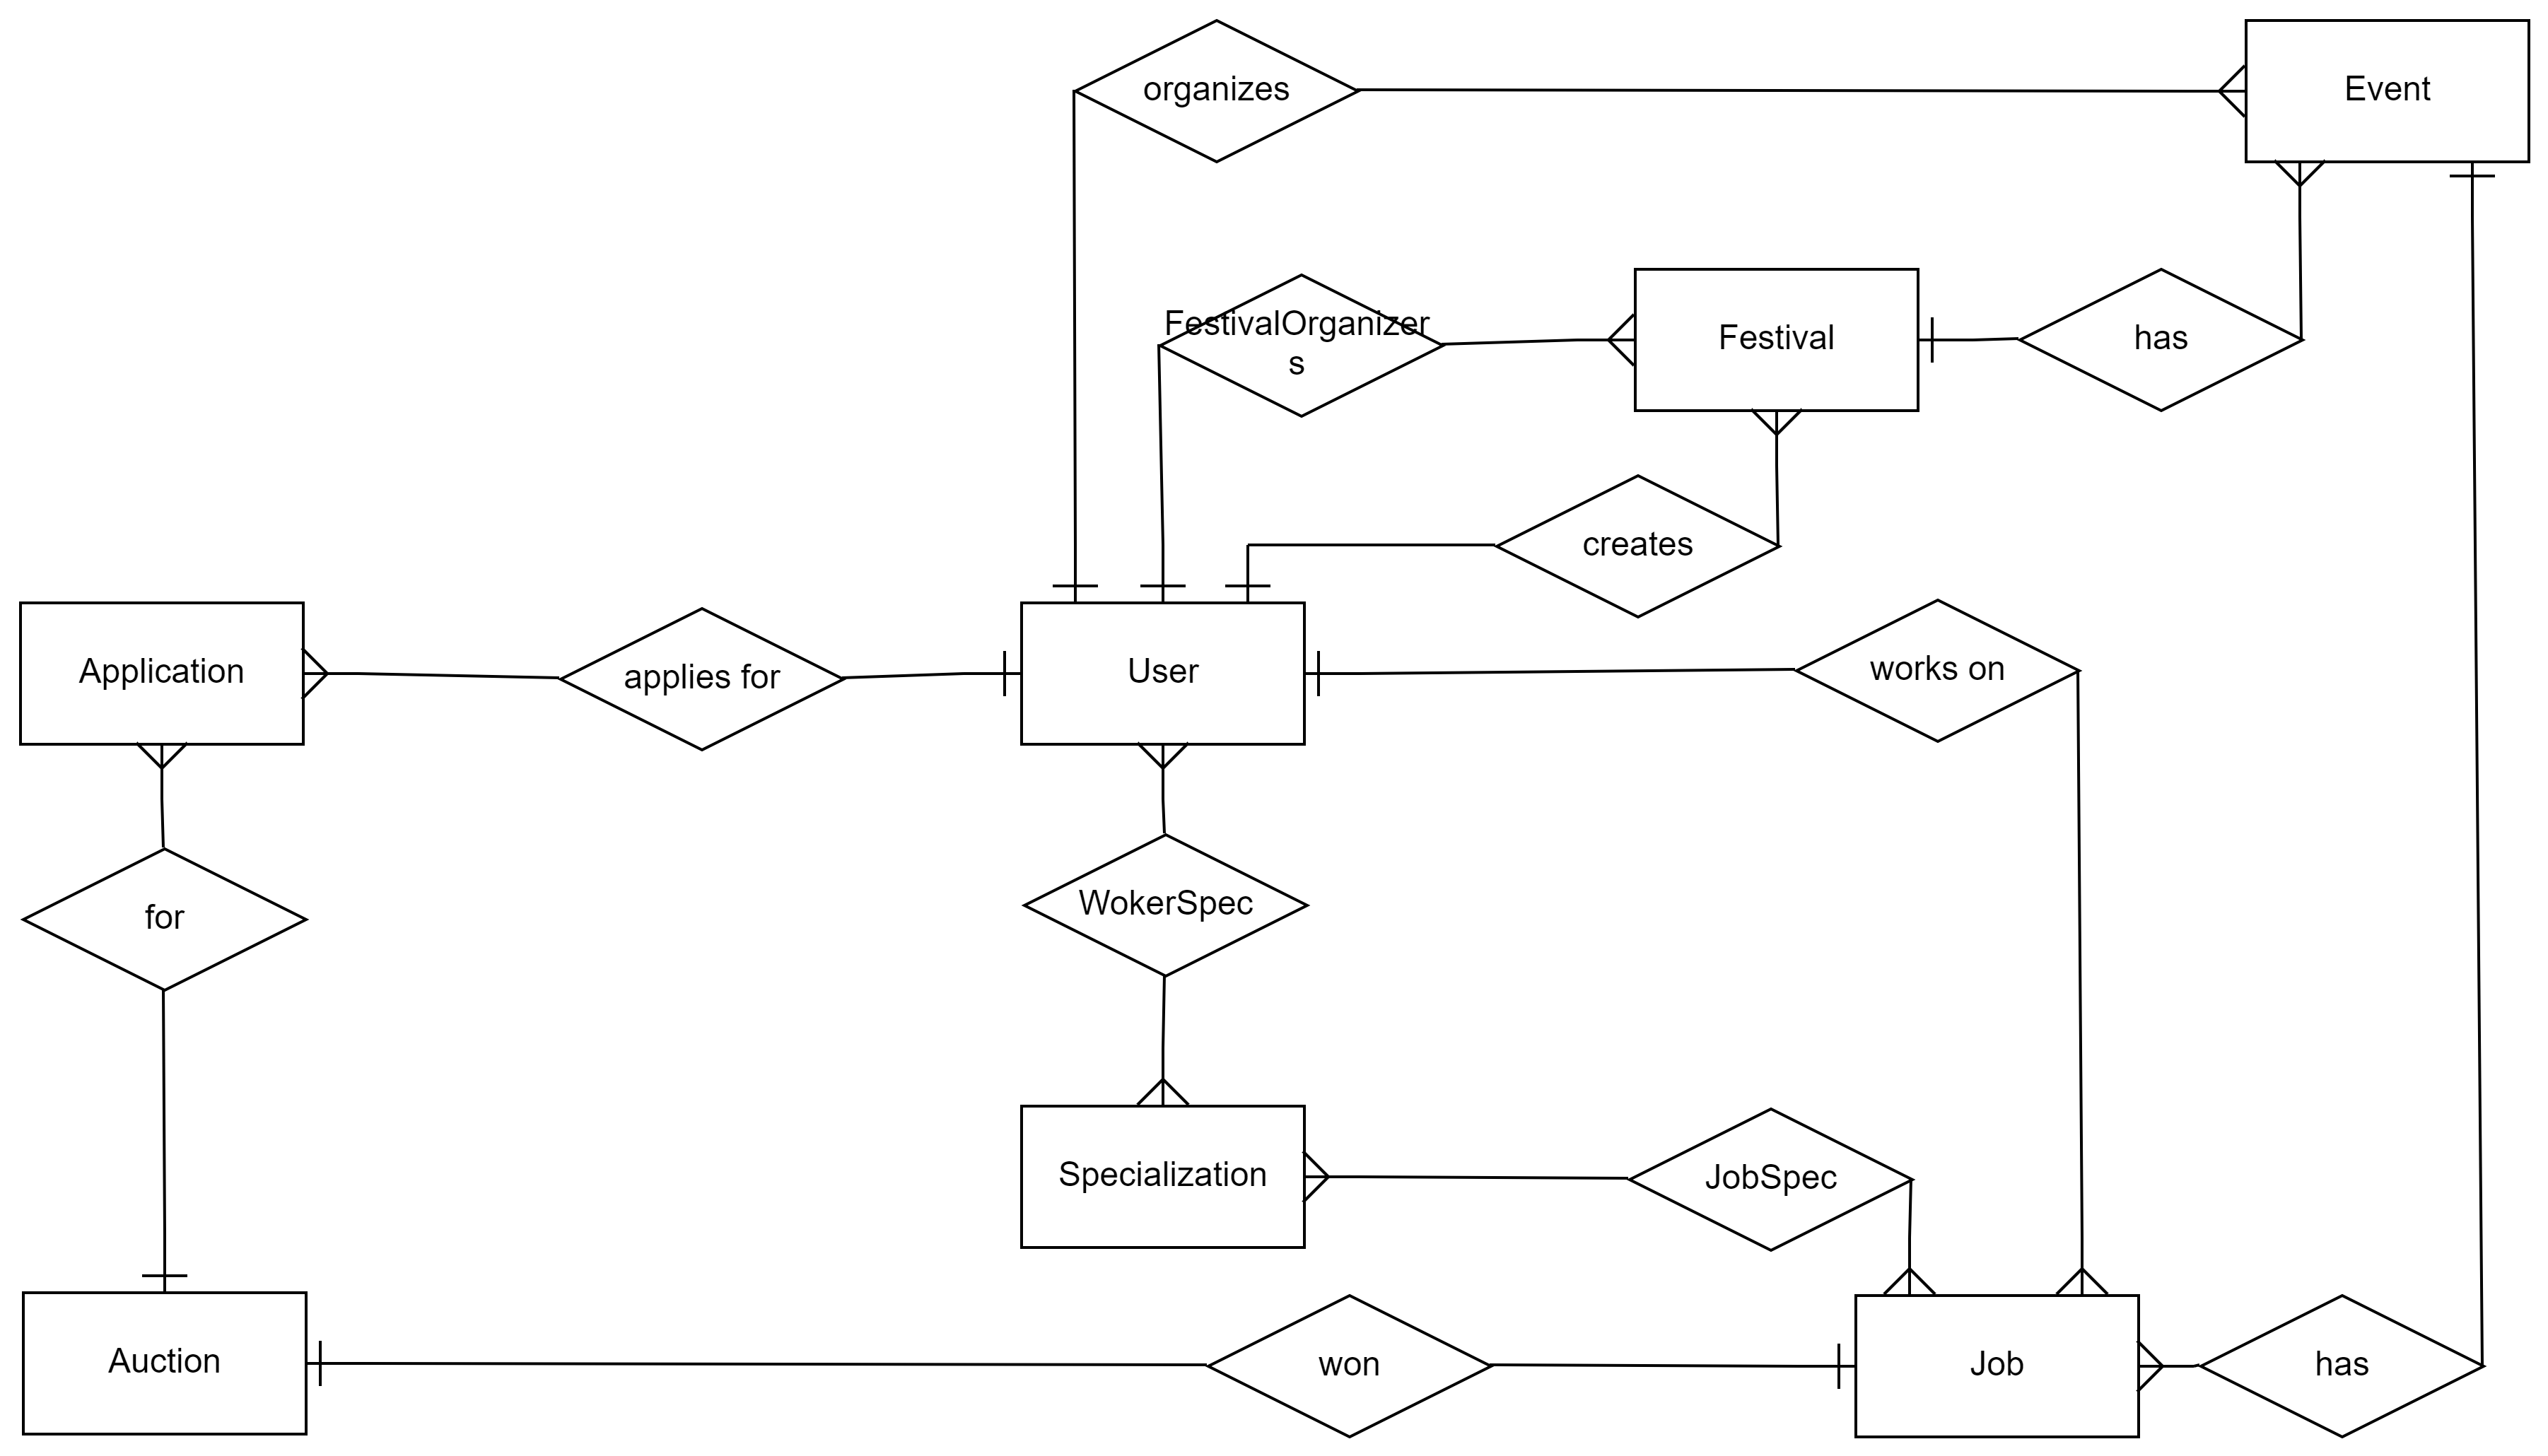
\includegraphics[width=\linewidth]{diagrams/db_er_diag.png}
					\centering
					\caption{E-R Diagram}
					\label{fig:er_diag}
				\end{figure}
			
				\begin{figure}[H]
					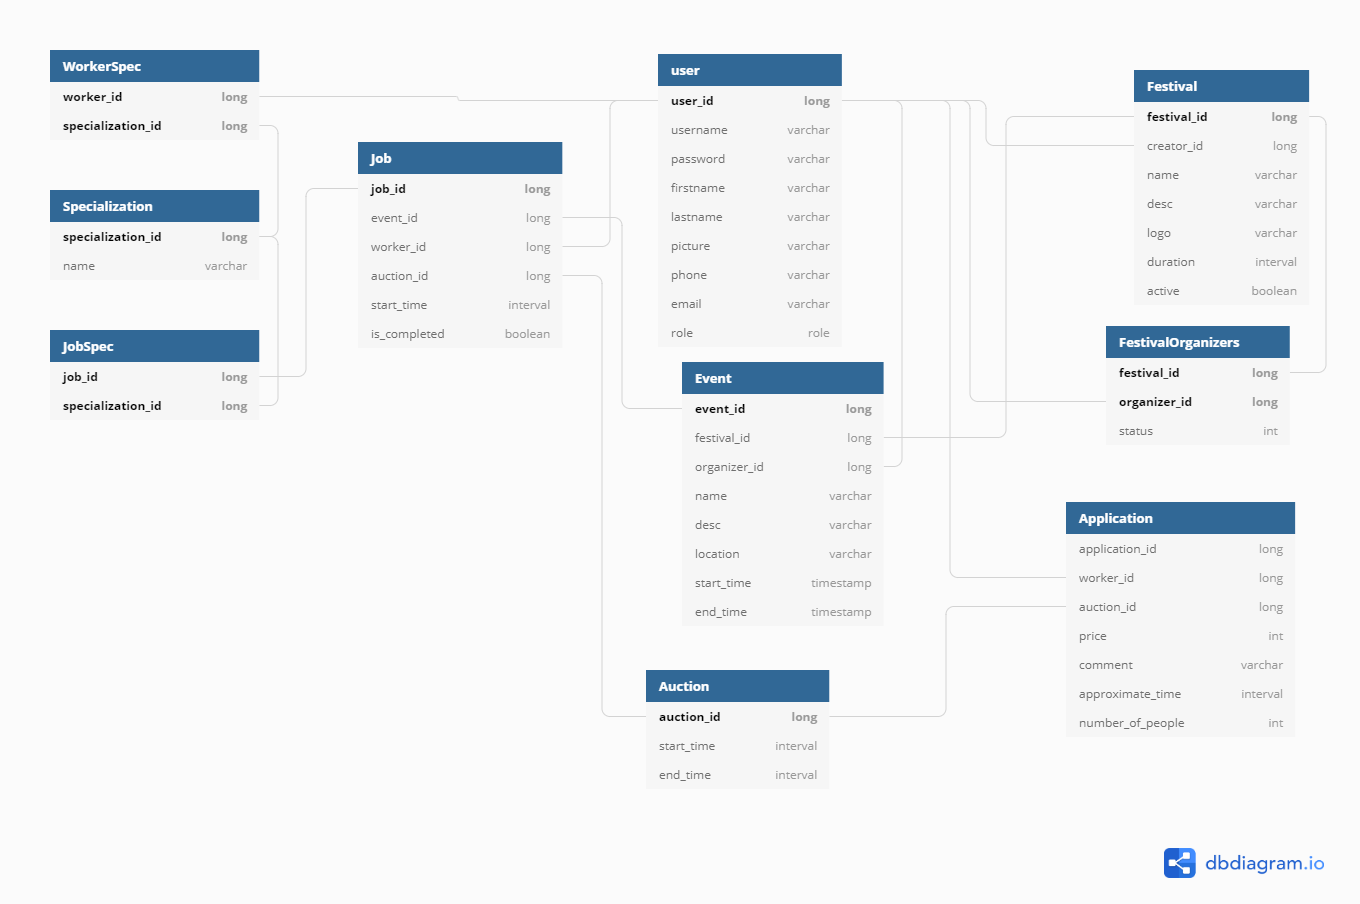
\includegraphics[width=\linewidth]{diagrams/db_normal_diag.png}
					\centering
					\caption{Database Diagram}
					\label{fig:normal_diag}
				\end{figure}
			
			\eject
			
			\pagebreak
		\section{Class Diagram}
			
			\begin{figure}[H]
				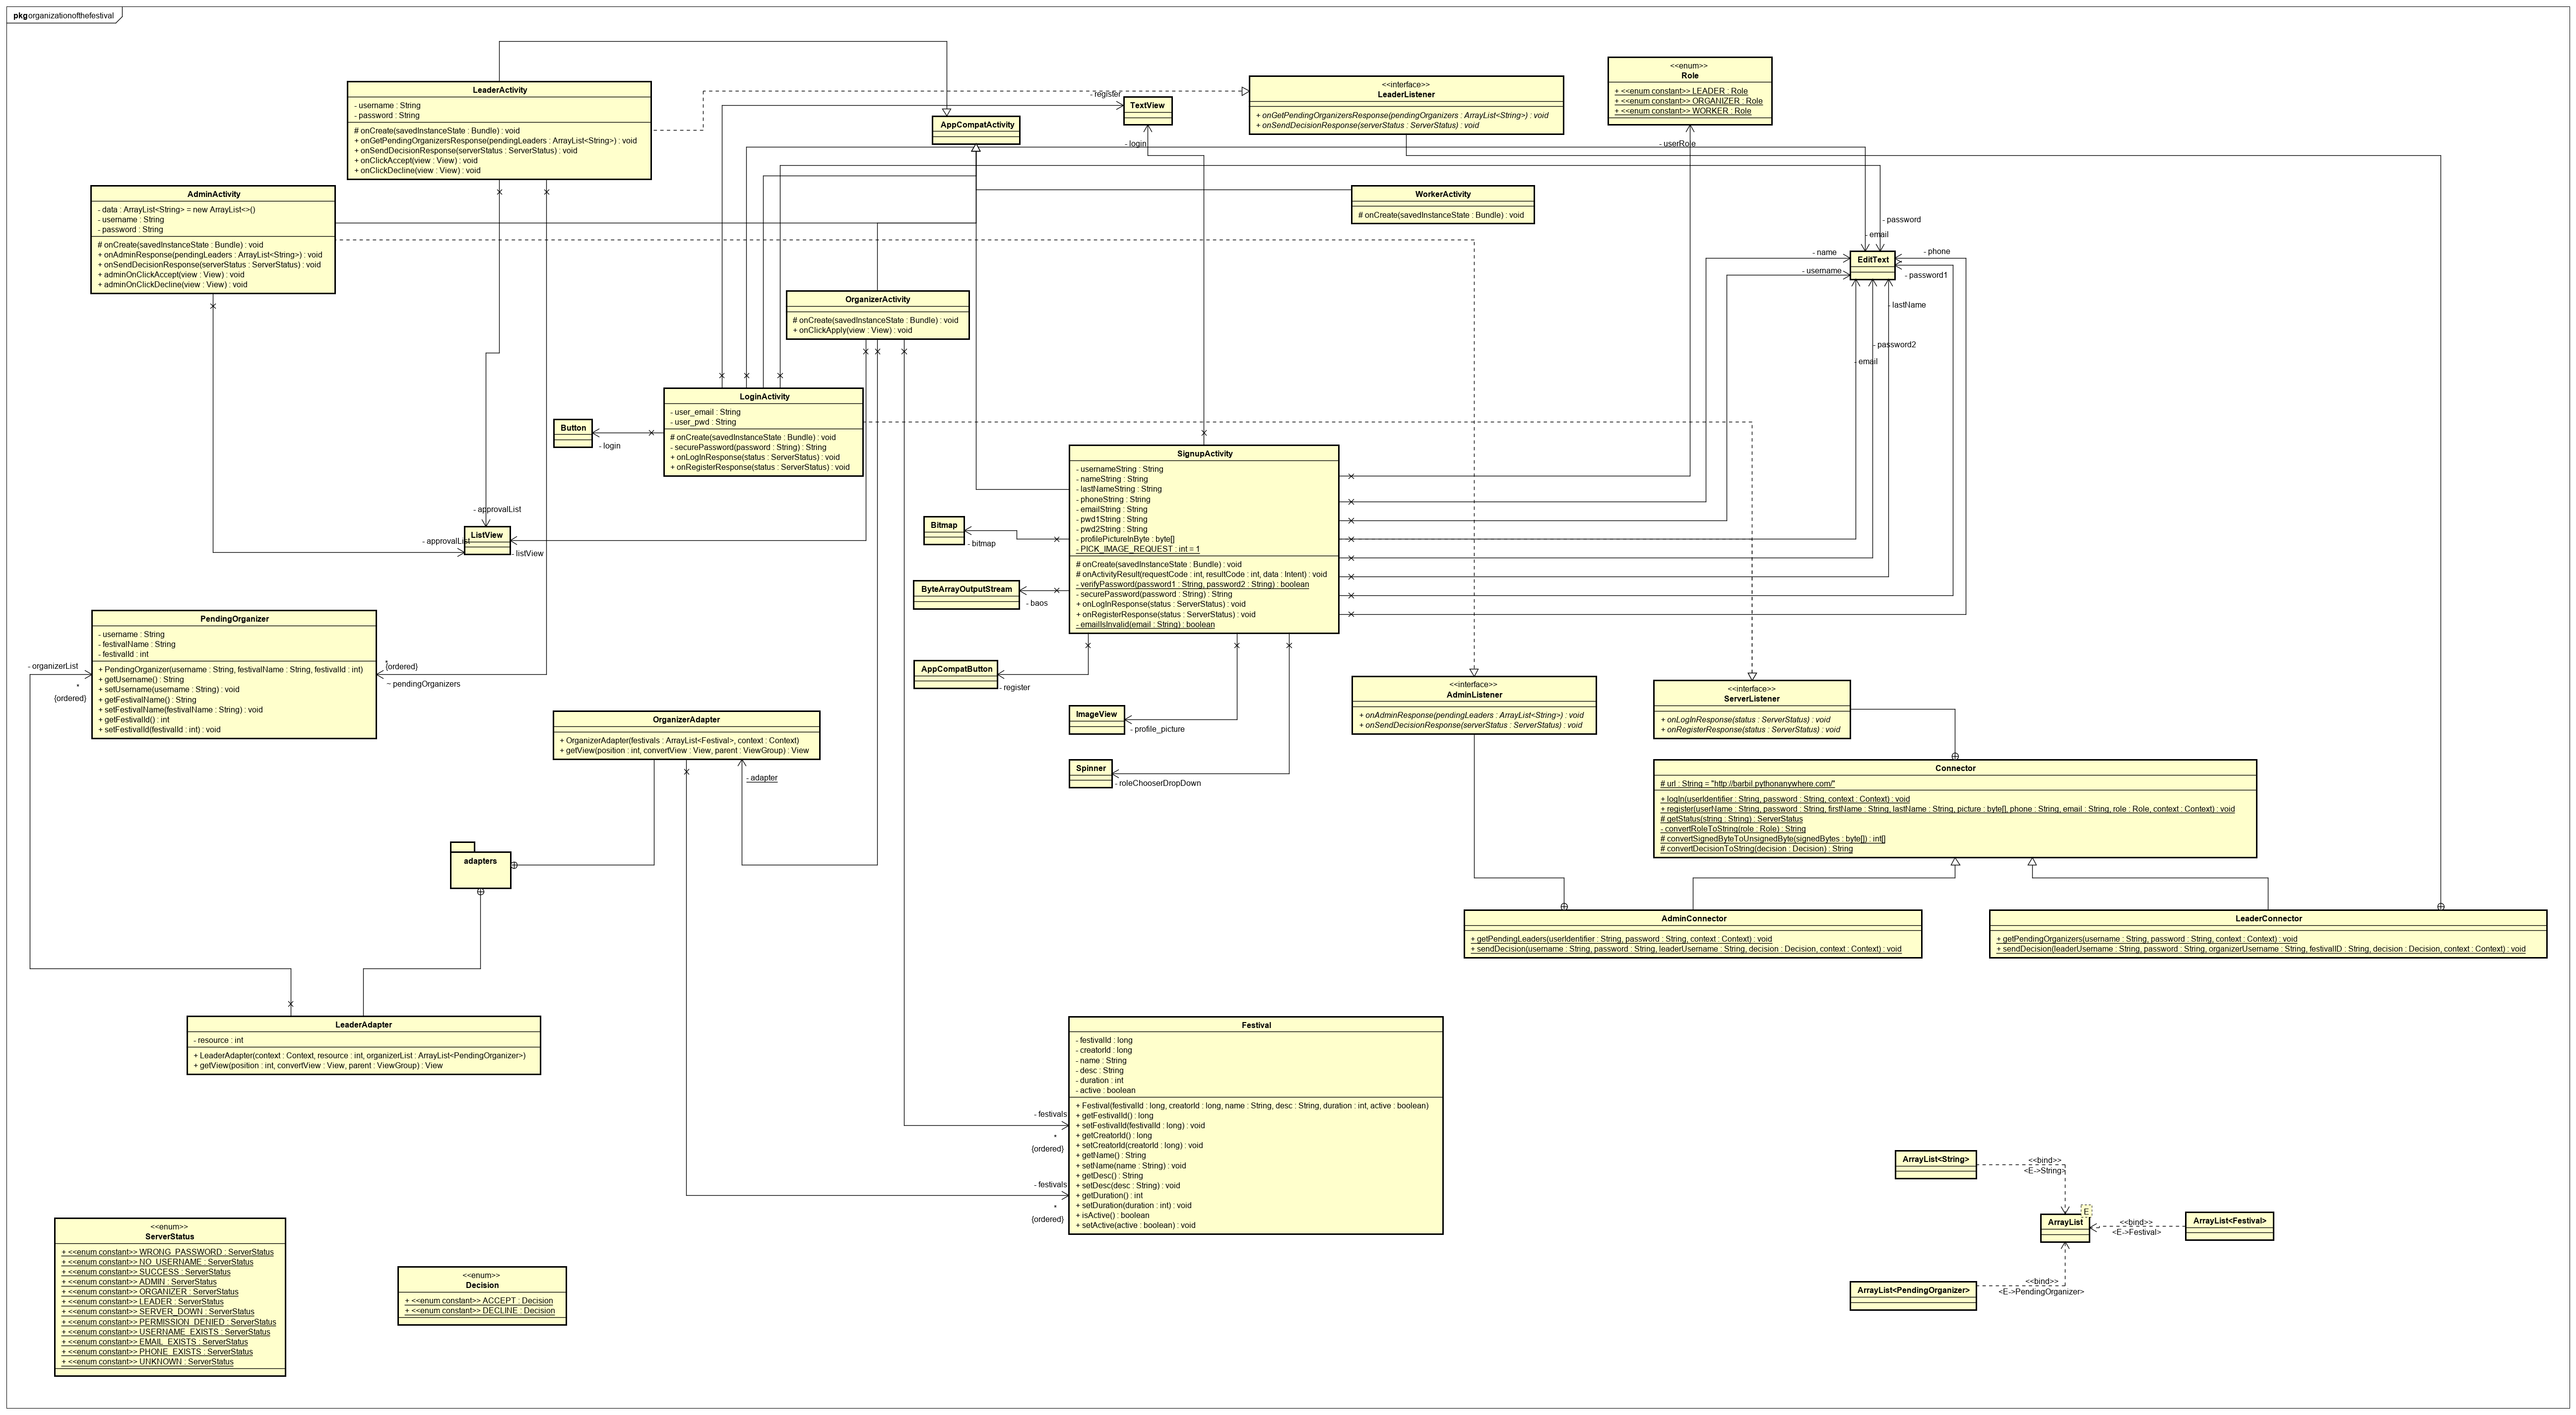
\includegraphics[width=\linewidth]{diagrams/UML-OrganizationOfTheFestival_v1.png}
				\caption{Class Diagram}
				\label{fig:class_diag}
			\end{figure}
			
			\textbf{ dio 2. revizije}\\			
			
			 Prilikom druge predaje projekta dijagram razreda i opisi moraju odgovarati stvarnom stanju implementacije
			
			
			
			\eject
		
		\section{Dijagram stanja}
			
			
			\textbf{ dio 2. revizije}\\
			
			 Potrebno je priložiti dijagram stanja i opisati ga. Dovoljan je jedan dijagram stanja koji prikazuje \textbf{značajan dio funkcionalnosti} sustava. Na primjer, stanja korisničkog sučelja i tijek korištenja neke ključne funkcionalnosti jesu značajan dio sustava, a registracija i prijava nisu. 
			
			
			\eject 
		
		\section{Dijagram aktivnosti}
			
			\textbf{ dio 2. revizije}\\
			
			  Potrebno je priložiti dijagram aktivnosti s pripadajućim opisom. Dijagram aktivnosti treba prikazivati značajan dio sustava.
			
			\eject
		\section{Dijagram komponenti}
		
			\textbf{ dio 2. revizije}\\
		
			  Potrebno je priložiti dijagram komponenti s pripadajućim opisom. Dijagram komponenti treba prikazivati strukturu cijele aplikacije.